% Created by tikzDevice version 0.7.0 on 2014-04-27 16:13:39
% !TEX encoding = UTF-8 Unicode
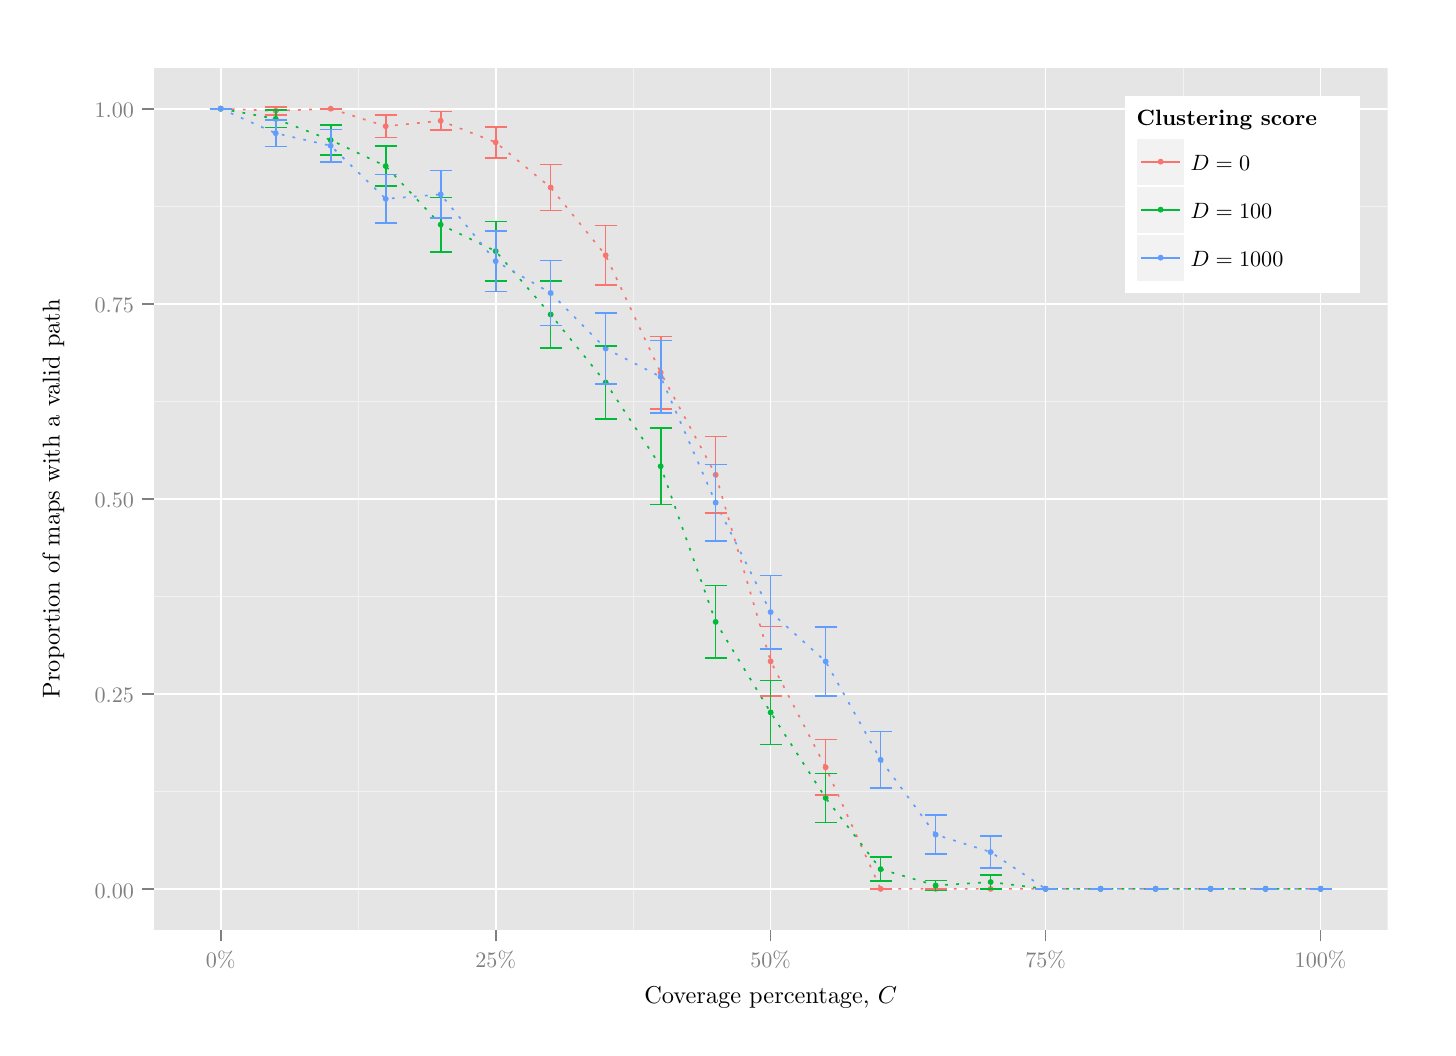
\begin{tikzpicture}[x=1pt,y=1pt]
\definecolor[named]{fillColor}{rgb}{1.00,1.00,1.00}
\path[use as bounding box,fill=fillColor,fill opacity=0.00] (0,0) rectangle (505.89,361.35);
\begin{scope}
\path[clip] (  0.00,  0.00) rectangle (505.89,361.35);
\definecolor[named]{drawColor}{rgb}{1.00,1.00,1.00}
\definecolor[named]{fillColor}{rgb}{1.00,1.00,1.00}

\path[draw=drawColor,line width= 0.6pt,line join=round,line cap=round,fill=fillColor] ( -0.00, -0.00) rectangle (505.89,361.35);
\end{scope}
\begin{scope}
\path[clip] ( 45.51, 35.41) rectangle (491.44,346.90);
\definecolor[named]{fillColor}{rgb}{0.90,0.90,0.90}

\path[fill=fillColor] ( 45.51, 35.41) rectangle (491.44,346.90);
\definecolor[named]{drawColor}{rgb}{0.95,0.95,0.95}

\path[draw=drawColor,line width= 0.3pt,line join=round] ( 45.51, 85.40) --
	(491.44, 85.40);

\path[draw=drawColor,line width= 0.3pt,line join=round] ( 45.51,155.87) --
	(491.44,155.87);

\path[draw=drawColor,line width= 0.3pt,line join=round] ( 45.51,226.35) --
	(491.44,226.35);

\path[draw=drawColor,line width= 0.3pt,line join=round] ( 45.51,296.83) --
	(491.44,296.83);

\path[draw=drawColor,line width= 0.3pt,line join=round] (119.43, 35.41) --
	(119.43,346.90);

\path[draw=drawColor,line width= 0.3pt,line join=round] (218.79, 35.41) --
	(218.79,346.90);

\path[draw=drawColor,line width= 0.3pt,line join=round] (318.15, 35.41) --
	(318.15,346.90);

\path[draw=drawColor,line width= 0.3pt,line join=round] (417.51, 35.41) --
	(417.51,346.90);
\definecolor[named]{drawColor}{rgb}{1.00,1.00,1.00}

\path[draw=drawColor,line width= 0.6pt,line join=round] ( 45.51, 50.16) --
	(491.44, 50.16);

\path[draw=drawColor,line width= 0.6pt,line join=round] ( 45.51,120.64) --
	(491.44,120.64);

\path[draw=drawColor,line width= 0.6pt,line join=round] ( 45.51,191.11) --
	(491.44,191.11);

\path[draw=drawColor,line width= 0.6pt,line join=round] ( 45.51,261.59) --
	(491.44,261.59);

\path[draw=drawColor,line width= 0.6pt,line join=round] ( 45.51,332.07) --
	(491.44,332.07);

\path[draw=drawColor,line width= 0.6pt,line join=round] ( 69.75, 35.41) --
	( 69.75,346.90);

\path[draw=drawColor,line width= 0.6pt,line join=round] (169.11, 35.41) --
	(169.11,346.90);

\path[draw=drawColor,line width= 0.6pt,line join=round] (268.47, 35.41) --
	(268.47,346.90);

\path[draw=drawColor,line width= 0.6pt,line join=round] (367.83, 35.41) --
	(367.83,346.90);

\path[draw=drawColor,line width= 0.6pt,line join=round] (467.19, 35.41) --
	(467.19,346.90);
\definecolor[named]{drawColor}{rgb}{0.97,0.46,0.43}

\path[draw=drawColor,line width= 0.6pt,dash pattern=on 1pt off 3pt ,line join=round] ( 69.75,332.07) --
	( 89.62,331.29) --
	(109.49,332.07) --
	(129.37,325.73) --
	(149.24,327.70) --
	(169.11,319.91) --
	(188.98,303.59) --
	(208.85,279.10) --
	(228.73,236.71) --
	(248.60,199.79) --
	(268.47,132.38) --
	(288.34, 94.09) --
	(308.22, 50.16) --
	(328.09, 50.16) --
	(347.96, 50.16) --
	(367.83, 50.16) --
	(387.70, 50.16) --
	(407.58, 50.16) --
	(427.45, 50.16) --
	(447.32, 50.16) --
	(467.19, 50.16);
\definecolor[named]{drawColor}{rgb}{0.00,0.73,0.22}

\path[draw=drawColor,line width= 0.6pt,dash pattern=on 1pt off 3pt ,line join=round] ( 69.75,332.07) --
	( 89.62,328.40) --
	(109.49,320.73) --
	(129.37,311.33) --
	(149.24,290.18) --
	(169.11,280.59) --
	(188.98,257.70) --
	(208.85,233.14) --
	(228.73,202.86) --
	(248.60,146.62) --
	(268.47,113.91) --
	(288.34, 83.01) --
	(308.22, 57.27) --
	(328.09, 51.39) --
	(347.96, 52.62) --
	(367.83, 50.16) --
	(387.70, 50.16) --
	(407.58, 50.16) --
	(427.45, 50.16) --
	(447.32, 50.16) --
	(467.19, 50.16);
\definecolor[named]{drawColor}{rgb}{0.38,0.61,1.00}

\path[draw=drawColor,line width= 0.6pt,dash pattern=on 1pt off 3pt ,line join=round] ( 69.75,332.07) --
	( 89.62,323.21) --
	(109.49,318.68) --
	(129.37,299.48) --
	(149.24,301.10) --
	(169.11,276.96) --
	(188.98,265.48) --
	(208.85,245.40) --
	(228.73,235.19) --
	(248.60,189.73) --
	(268.47,150.16) --
	(288.34,132.33) --
	(308.22, 96.79) --
	(328.09, 69.77) --
	(347.96, 63.46) --
	(367.83, 50.16) --
	(387.70, 50.16) --
	(407.58, 50.16) --
	(427.45, 50.16) --
	(447.32, 50.16) --
	(467.19, 50.16);
\definecolor[named]{fillColor}{rgb}{0.97,0.46,0.43}

\path[fill=fillColor] ( 69.75,332.07) circle (  1.07);

\path[fill=fillColor] ( 89.62,331.29) circle (  1.07);

\path[fill=fillColor] (109.49,332.07) circle (  1.07);

\path[fill=fillColor] (129.37,325.73) circle (  1.07);

\path[fill=fillColor] (149.24,327.70) circle (  1.07);

\path[fill=fillColor] (169.11,319.91) circle (  1.07);

\path[fill=fillColor] (188.98,303.59) circle (  1.07);

\path[fill=fillColor] (208.85,279.10) circle (  1.07);

\path[fill=fillColor] (228.73,236.71) circle (  1.07);

\path[fill=fillColor] (248.60,199.79) circle (  1.07);

\path[fill=fillColor] (268.47,132.38) circle (  1.07);

\path[fill=fillColor] (288.34, 94.09) circle (  1.07);

\path[fill=fillColor] (308.22, 50.16) circle (  1.07);

\path[fill=fillColor] (328.09, 50.16) circle (  1.07);

\path[fill=fillColor] (347.96, 50.16) circle (  1.07);

\path[fill=fillColor] (367.83, 50.16) circle (  1.07);

\path[fill=fillColor] (387.70, 50.16) circle (  1.07);

\path[fill=fillColor] (407.58, 50.16) circle (  1.07);

\path[fill=fillColor] (427.45, 50.16) circle (  1.07);

\path[fill=fillColor] (447.32, 50.16) circle (  1.07);

\path[fill=fillColor] (467.19, 50.16) circle (  1.07);
\definecolor[named]{fillColor}{rgb}{0.00,0.73,0.22}

\path[fill=fillColor] ( 69.75,332.07) circle (  1.07);

\path[fill=fillColor] ( 89.62,328.40) circle (  1.07);

\path[fill=fillColor] (109.49,320.73) circle (  1.07);

\path[fill=fillColor] (129.37,311.33) circle (  1.07);

\path[fill=fillColor] (149.24,290.18) circle (  1.07);

\path[fill=fillColor] (169.11,280.59) circle (  1.07);

\path[fill=fillColor] (188.98,257.70) circle (  1.07);

\path[fill=fillColor] (208.85,233.14) circle (  1.07);

\path[fill=fillColor] (228.73,202.86) circle (  1.07);

\path[fill=fillColor] (248.60,146.62) circle (  1.07);

\path[fill=fillColor] (268.47,113.91) circle (  1.07);

\path[fill=fillColor] (288.34, 83.01) circle (  1.07);

\path[fill=fillColor] (308.22, 57.27) circle (  1.07);

\path[fill=fillColor] (328.09, 51.39) circle (  1.07);

\path[fill=fillColor] (347.96, 52.62) circle (  1.07);

\path[fill=fillColor] (367.83, 50.16) circle (  1.07);

\path[fill=fillColor] (387.70, 50.16) circle (  1.07);

\path[fill=fillColor] (407.58, 50.16) circle (  1.07);

\path[fill=fillColor] (427.45, 50.16) circle (  1.07);

\path[fill=fillColor] (447.32, 50.16) circle (  1.07);

\path[fill=fillColor] (467.19, 50.16) circle (  1.07);
\definecolor[named]{fillColor}{rgb}{0.38,0.61,1.00}

\path[fill=fillColor] ( 69.75,332.07) circle (  1.07);

\path[fill=fillColor] ( 89.62,323.21) circle (  1.07);

\path[fill=fillColor] (109.49,318.68) circle (  1.07);

\path[fill=fillColor] (129.37,299.48) circle (  1.07);

\path[fill=fillColor] (149.24,301.10) circle (  1.07);

\path[fill=fillColor] (169.11,276.96) circle (  1.07);

\path[fill=fillColor] (188.98,265.48) circle (  1.07);

\path[fill=fillColor] (208.85,245.40) circle (  1.07);

\path[fill=fillColor] (228.73,235.19) circle (  1.07);

\path[fill=fillColor] (248.60,189.73) circle (  1.07);

\path[fill=fillColor] (268.47,150.16) circle (  1.07);

\path[fill=fillColor] (288.34,132.33) circle (  1.07);

\path[fill=fillColor] (308.22, 96.79) circle (  1.07);

\path[fill=fillColor] (328.09, 69.77) circle (  1.07);

\path[fill=fillColor] (347.96, 63.46) circle (  1.07);

\path[fill=fillColor] (367.83, 50.16) circle (  1.07);

\path[fill=fillColor] (387.70, 50.16) circle (  1.07);

\path[fill=fillColor] (407.58, 50.16) circle (  1.07);

\path[fill=fillColor] (427.45, 50.16) circle (  1.07);

\path[fill=fillColor] (447.32, 50.16) circle (  1.07);

\path[fill=fillColor] (467.19, 50.16) circle (  1.07);
\definecolor[named]{drawColor}{rgb}{0.97,0.46,0.43}

\path[draw=drawColor,line width= 0.6pt,line join=round] ( 65.78,332.07) --
	( 73.72,332.07);

\path[draw=drawColor,line width= 0.6pt,line join=round] ( 69.75,332.07) --
	( 69.75,332.07);

\path[draw=drawColor,line width= 0.6pt,line join=round] ( 65.78,332.07) --
	( 73.72,332.07);

\path[draw=drawColor,line width= 0.6pt,line join=round] ( 85.65,332.74) --
	( 93.60,332.74);

\path[draw=drawColor,line width= 0.6pt,line join=round] ( 89.62,332.74) --
	( 89.62,329.85);

\path[draw=drawColor,line width= 0.6pt,line join=round] ( 85.65,329.85) --
	( 93.60,329.85);

\path[draw=drawColor,line width= 0.6pt,line join=round] (105.52,332.07) --
	(113.47,332.07);

\path[draw=drawColor,line width= 0.6pt,line join=round] (109.49,332.07) --
	(109.49,332.07);

\path[draw=drawColor,line width= 0.6pt,line join=round] (105.52,332.07) --
	(113.47,332.07);

\path[draw=drawColor,line width= 0.6pt,line join=round] (125.39,329.83) --
	(133.34,329.83);

\path[draw=drawColor,line width= 0.6pt,line join=round] (129.37,329.83) --
	(129.37,321.64);

\path[draw=drawColor,line width= 0.6pt,line join=round] (125.39,321.64) --
	(133.34,321.64);

\path[draw=drawColor,line width= 0.6pt,line join=round] (145.26,331.11) --
	(153.21,331.11);

\path[draw=drawColor,line width= 0.6pt,line join=round] (149.24,331.11) --
	(149.24,324.28);

\path[draw=drawColor,line width= 0.6pt,line join=round] (145.26,324.28) --
	(153.21,324.28);

\path[draw=drawColor,line width= 0.6pt,line join=round] (165.14,325.53) --
	(173.08,325.53);

\path[draw=drawColor,line width= 0.6pt,line join=round] (169.11,325.53) --
	(169.11,314.30);

\path[draw=drawColor,line width= 0.6pt,line join=round] (165.14,314.30) --
	(173.08,314.30);

\path[draw=drawColor,line width= 0.6pt,line join=round] (185.01,311.92) --
	(192.96,311.92);

\path[draw=drawColor,line width= 0.6pt,line join=round] (188.98,311.92) --
	(188.98,295.27);

\path[draw=drawColor,line width= 0.6pt,line join=round] (185.01,295.27) --
	(192.96,295.27);

\path[draw=drawColor,line width= 0.6pt,line join=round] (204.88,289.89) --
	(212.83,289.89);

\path[draw=drawColor,line width= 0.6pt,line join=round] (208.85,289.89) --
	(208.85,268.31);

\path[draw=drawColor,line width= 0.6pt,line join=round] (204.88,268.31) --
	(212.83,268.31);

\path[draw=drawColor,line width= 0.6pt,line join=round] (224.75,249.79) --
	(232.70,249.79);

\path[draw=drawColor,line width= 0.6pt,line join=round] (228.73,249.79) --
	(228.73,223.64);

\path[draw=drawColor,line width= 0.6pt,line join=round] (224.75,223.64) --
	(232.70,223.64);

\path[draw=drawColor,line width= 0.6pt,line join=round] (244.62,213.57) --
	(252.57,213.57);

\path[draw=drawColor,line width= 0.6pt,line join=round] (248.60,213.57) --
	(248.60,186.00);

\path[draw=drawColor,line width= 0.6pt,line join=round] (244.62,186.00) --
	(252.57,186.00);

\path[draw=drawColor,line width= 0.6pt,line join=round] (264.50,144.94) --
	(272.45,144.94);

\path[draw=drawColor,line width= 0.6pt,line join=round] (268.47,144.94) --
	(268.47,119.82);

\path[draw=drawColor,line width= 0.6pt,line join=round] (264.50,119.82) --
	(272.45,119.82);

\path[draw=drawColor,line width= 0.6pt,line join=round] (284.37,104.11) --
	(292.32,104.11);

\path[draw=drawColor,line width= 0.6pt,line join=round] (288.34,104.11) --
	(288.34, 84.07);

\path[draw=drawColor,line width= 0.6pt,line join=round] (284.37, 84.07) --
	(292.32, 84.07);

\path[draw=drawColor,line width= 0.6pt,line join=round] (304.24, 50.16) --
	(312.19, 50.16);

\path[draw=drawColor,line width= 0.6pt,line join=round] (308.22, 50.16) --
	(308.22, 50.16);

\path[draw=drawColor,line width= 0.6pt,line join=round] (304.24, 50.16) --
	(312.19, 50.16);

\path[draw=drawColor,line width= 0.6pt,line join=round] (324.11, 50.16) --
	(332.06, 50.16);

\path[draw=drawColor,line width= 0.6pt,line join=round] (328.09, 50.16) --
	(328.09, 50.16);

\path[draw=drawColor,line width= 0.6pt,line join=round] (324.11, 50.16) --
	(332.06, 50.16);

\path[draw=drawColor,line width= 0.6pt,line join=round] (343.98, 50.16) --
	(351.93, 50.16);

\path[draw=drawColor,line width= 0.6pt,line join=round] (347.96, 50.16) --
	(347.96, 50.16);

\path[draw=drawColor,line width= 0.6pt,line join=round] (343.98, 50.16) --
	(351.93, 50.16);

\path[draw=drawColor,line width= 0.6pt,line join=round] (363.86, 50.16) --
	(371.81, 50.16);

\path[draw=drawColor,line width= 0.6pt,line join=round] (367.83, 50.16) --
	(367.83, 50.16);

\path[draw=drawColor,line width= 0.6pt,line join=round] (363.86, 50.16) --
	(371.81, 50.16);

\path[draw=drawColor,line width= 0.6pt,line join=round] (383.73, 50.16) --
	(391.68, 50.16);

\path[draw=drawColor,line width= 0.6pt,line join=round] (387.70, 50.16) --
	(387.70, 50.16);

\path[draw=drawColor,line width= 0.6pt,line join=round] (383.73, 50.16) --
	(391.68, 50.16);

\path[draw=drawColor,line width= 0.6pt,line join=round] (403.60, 50.16) --
	(411.55, 50.16);

\path[draw=drawColor,line width= 0.6pt,line join=round] (407.58, 50.16) --
	(407.58, 50.16);

\path[draw=drawColor,line width= 0.6pt,line join=round] (403.60, 50.16) --
	(411.55, 50.16);

\path[draw=drawColor,line width= 0.6pt,line join=round] (423.47, 50.16) --
	(431.42, 50.16);

\path[draw=drawColor,line width= 0.6pt,line join=round] (427.45, 50.16) --
	(427.45, 50.16);

\path[draw=drawColor,line width= 0.6pt,line join=round] (423.47, 50.16) --
	(431.42, 50.16);

\path[draw=drawColor,line width= 0.6pt,line join=round] (443.35, 50.16) --
	(451.29, 50.16);

\path[draw=drawColor,line width= 0.6pt,line join=round] (447.32, 50.16) --
	(447.32, 50.16);

\path[draw=drawColor,line width= 0.6pt,line join=round] (443.35, 50.16) --
	(451.29, 50.16);

\path[draw=drawColor,line width= 0.6pt,line join=round] (463.22, 50.16) --
	(471.17, 50.16);

\path[draw=drawColor,line width= 0.6pt,line join=round] (467.19, 50.16) --
	(467.19, 50.16);

\path[draw=drawColor,line width= 0.6pt,line join=round] (463.22, 50.16) --
	(471.17, 50.16);
\definecolor[named]{drawColor}{rgb}{0.00,0.73,0.22}

\path[draw=drawColor,line width= 0.6pt,line join=round] ( 65.78,332.07) --
	( 73.72,332.07);

\path[draw=drawColor,line width= 0.6pt,line join=round] ( 69.75,332.07) --
	( 69.75,332.07);

\path[draw=drawColor,line width= 0.6pt,line join=round] ( 65.78,332.07) --
	( 73.72,332.07);

\path[draw=drawColor,line width= 0.6pt,line join=round] ( 85.65,331.53) --
	( 93.60,331.53);

\path[draw=drawColor,line width= 0.6pt,line join=round] ( 89.62,331.53) --
	( 89.62,325.26);

\path[draw=drawColor,line width= 0.6pt,line join=round] ( 85.65,325.26) --
	( 93.60,325.26);

\path[draw=drawColor,line width= 0.6pt,line join=round] (105.52,326.16) --
	(113.47,326.16);

\path[draw=drawColor,line width= 0.6pt,line join=round] (109.49,326.16) --
	(109.49,315.30);

\path[draw=drawColor,line width= 0.6pt,line join=round] (105.52,315.30) --
	(113.47,315.30);

\path[draw=drawColor,line width= 0.6pt,line join=round] (125.39,318.54) --
	(133.34,318.54);

\path[draw=drawColor,line width= 0.6pt,line join=round] (129.37,318.54) --
	(129.37,304.11);

\path[draw=drawColor,line width= 0.6pt,line join=round] (125.39,304.11) --
	(133.34,304.11);

\path[draw=drawColor,line width= 0.6pt,line join=round] (145.26,300.01) --
	(153.21,300.01);

\path[draw=drawColor,line width= 0.6pt,line join=round] (149.24,300.01) --
	(149.24,280.36);

\path[draw=drawColor,line width= 0.6pt,line join=round] (145.26,280.36) --
	(153.21,280.36);

\path[draw=drawColor,line width= 0.6pt,line join=round] (165.14,291.26) --
	(173.08,291.26);

\path[draw=drawColor,line width= 0.6pt,line join=round] (169.11,291.26) --
	(169.11,269.91);

\path[draw=drawColor,line width= 0.6pt,line join=round] (165.14,269.91) --
	(173.08,269.91);

\path[draw=drawColor,line width= 0.6pt,line join=round] (185.01,269.87) --
	(192.96,269.87);

\path[draw=drawColor,line width= 0.6pt,line join=round] (188.98,269.87) --
	(188.98,245.52);

\path[draw=drawColor,line width= 0.6pt,line join=round] (185.01,245.52) --
	(192.96,245.52);

\path[draw=drawColor,line width= 0.6pt,line join=round] (204.88,246.32) --
	(212.83,246.32);

\path[draw=drawColor,line width= 0.6pt,line join=round] (208.85,246.32) --
	(208.85,219.95);

\path[draw=drawColor,line width= 0.6pt,line join=round] (204.88,219.95) --
	(212.83,219.95);

\path[draw=drawColor,line width= 0.6pt,line join=round] (224.75,216.62) --
	(232.70,216.62);

\path[draw=drawColor,line width= 0.6pt,line join=round] (228.73,216.62) --
	(228.73,189.09);

\path[draw=drawColor,line width= 0.6pt,line join=round] (224.75,189.09) --
	(232.70,189.09);

\path[draw=drawColor,line width= 0.6pt,line join=round] (244.62,159.73) --
	(252.57,159.73);

\path[draw=drawColor,line width= 0.6pt,line join=round] (248.60,159.73) --
	(248.60,133.52);

\path[draw=drawColor,line width= 0.6pt,line join=round] (244.62,133.52) --
	(252.57,133.52);

\path[draw=drawColor,line width= 0.6pt,line join=round] (264.50,125.47) --
	(272.45,125.47);

\path[draw=drawColor,line width= 0.6pt,line join=round] (268.47,125.47) --
	(268.47,102.35);

\path[draw=drawColor,line width= 0.6pt,line join=round] (264.50,102.35) --
	(272.45,102.35);

\path[draw=drawColor,line width= 0.6pt,line join=round] (284.37, 91.88) --
	(292.32, 91.88);

\path[draw=drawColor,line width= 0.6pt,line join=round] (288.34, 91.88) --
	(288.34, 74.15);

\path[draw=drawColor,line width= 0.6pt,line join=round] (284.37, 74.15) --
	(292.32, 74.15);

\path[draw=drawColor,line width= 0.6pt,line join=round] (304.24, 61.60) --
	(312.19, 61.60);

\path[draw=drawColor,line width= 0.6pt,line join=round] (308.22, 61.60) --
	(308.22, 52.93);

\path[draw=drawColor,line width= 0.6pt,line join=round] (304.24, 52.93) --
	(312.19, 52.93);

\path[draw=drawColor,line width= 0.6pt,line join=round] (324.11, 53.22) --
	(332.06, 53.22);

\path[draw=drawColor,line width= 0.6pt,line join=round] (328.09, 53.22) --
	(328.09, 49.57);

\path[draw=drawColor,line width= 0.6pt,line join=round] (324.11, 49.57) --
	(332.06, 49.57);

\path[draw=drawColor,line width= 0.6pt,line join=round] (343.98, 55.19) --
	(351.93, 55.19);

\path[draw=drawColor,line width= 0.6pt,line join=round] (347.96, 55.19) --
	(347.96, 50.05);

\path[draw=drawColor,line width= 0.6pt,line join=round] (343.98, 50.05) --
	(351.93, 50.05);

\path[draw=drawColor,line width= 0.6pt,line join=round] (363.86, 50.16) --
	(371.81, 50.16);

\path[draw=drawColor,line width= 0.6pt,line join=round] (367.83, 50.16) --
	(367.83, 50.16);

\path[draw=drawColor,line width= 0.6pt,line join=round] (363.86, 50.16) --
	(371.81, 50.16);

\path[draw=drawColor,line width= 0.6pt,line join=round] (383.73, 50.16) --
	(391.68, 50.16);

\path[draw=drawColor,line width= 0.6pt,line join=round] (387.70, 50.16) --
	(387.70, 50.16);

\path[draw=drawColor,line width= 0.6pt,line join=round] (383.73, 50.16) --
	(391.68, 50.16);

\path[draw=drawColor,line width= 0.6pt,line join=round] (403.60, 50.16) --
	(411.55, 50.16);

\path[draw=drawColor,line width= 0.6pt,line join=round] (407.58, 50.16) --
	(407.58, 50.16);

\path[draw=drawColor,line width= 0.6pt,line join=round] (403.60, 50.16) --
	(411.55, 50.16);

\path[draw=drawColor,line width= 0.6pt,line join=round] (423.47, 50.16) --
	(431.42, 50.16);

\path[draw=drawColor,line width= 0.6pt,line join=round] (427.45, 50.16) --
	(427.45, 50.16);

\path[draw=drawColor,line width= 0.6pt,line join=round] (423.47, 50.16) --
	(431.42, 50.16);

\path[draw=drawColor,line width= 0.6pt,line join=round] (443.35, 50.16) --
	(451.29, 50.16);

\path[draw=drawColor,line width= 0.6pt,line join=round] (447.32, 50.16) --
	(447.32, 50.16);

\path[draw=drawColor,line width= 0.6pt,line join=round] (443.35, 50.16) --
	(451.29, 50.16);

\path[draw=drawColor,line width= 0.6pt,line join=round] (463.22, 50.16) --
	(471.17, 50.16);

\path[draw=drawColor,line width= 0.6pt,line join=round] (467.19, 50.16) --
	(467.19, 50.16);

\path[draw=drawColor,line width= 0.6pt,line join=round] (463.22, 50.16) --
	(471.17, 50.16);
\definecolor[named]{drawColor}{rgb}{0.38,0.61,1.00}

\path[draw=drawColor,line width= 0.6pt,line join=round] ( 65.78,332.07) --
	( 73.72,332.07);

\path[draw=drawColor,line width= 0.6pt,line join=round] ( 69.75,332.07) --
	( 69.75,332.07);

\path[draw=drawColor,line width= 0.6pt,line join=round] ( 65.78,332.07) --
	( 73.72,332.07);

\path[draw=drawColor,line width= 0.6pt,line join=round] ( 85.65,328.03) --
	( 93.60,328.03);

\path[draw=drawColor,line width= 0.6pt,line join=round] ( 89.62,328.03) --
	( 89.62,318.39);

\path[draw=drawColor,line width= 0.6pt,line join=round] ( 85.65,318.39) --
	( 93.60,318.39);

\path[draw=drawColor,line width= 0.6pt,line join=round] (105.52,324.55) --
	(113.47,324.55);

\path[draw=drawColor,line width= 0.6pt,line join=round] (109.49,324.55) --
	(109.49,312.80);

\path[draw=drawColor,line width= 0.6pt,line join=round] (105.52,312.80) --
	(113.47,312.80);

\path[draw=drawColor,line width= 0.6pt,line join=round] (125.39,308.31) --
	(133.34,308.31);

\path[draw=drawColor,line width= 0.6pt,line join=round] (129.37,308.31) --
	(129.37,290.65);

\path[draw=drawColor,line width= 0.6pt,line join=round] (125.39,290.65) --
	(133.34,290.65);

\path[draw=drawColor,line width= 0.6pt,line join=round] (145.26,309.74) --
	(153.21,309.74);

\path[draw=drawColor,line width= 0.6pt,line join=round] (149.24,309.74) --
	(149.24,292.46);

\path[draw=drawColor,line width= 0.6pt,line join=round] (145.26,292.46) --
	(153.21,292.46);

\path[draw=drawColor,line width= 0.6pt,line join=round] (165.14,287.92) --
	(173.08,287.92);

\path[draw=drawColor,line width= 0.6pt,line join=round] (169.11,287.92) --
	(169.11,266.01);

\path[draw=drawColor,line width= 0.6pt,line join=round] (165.14,266.01) --
	(173.08,266.01);

\path[draw=drawColor,line width= 0.6pt,line join=round] (185.01,277.21) --
	(192.96,277.21);

\path[draw=drawColor,line width= 0.6pt,line join=round] (188.98,277.21) --
	(188.98,253.75);

\path[draw=drawColor,line width= 0.6pt,line join=round] (185.01,253.75) --
	(192.96,253.75);

\path[draw=drawColor,line width= 0.6pt,line join=round] (204.88,258.14) --
	(212.83,258.14);

\path[draw=drawColor,line width= 0.6pt,line join=round] (208.85,258.14) --
	(208.85,232.65);

\path[draw=drawColor,line width= 0.6pt,line join=round] (204.88,232.65) --
	(212.83,232.65);

\path[draw=drawColor,line width= 0.6pt,line join=round] (224.75,248.31) --
	(232.70,248.31);

\path[draw=drawColor,line width= 0.6pt,line join=round] (228.73,248.31) --
	(228.73,222.07);

\path[draw=drawColor,line width= 0.6pt,line join=round] (224.75,222.07) --
	(232.70,222.07);

\path[draw=drawColor,line width= 0.6pt,line join=round] (244.62,203.54) --
	(252.57,203.54);

\path[draw=drawColor,line width= 0.6pt,line join=round] (248.60,203.54) --
	(248.60,175.91);

\path[draw=drawColor,line width= 0.6pt,line join=round] (244.62,175.91) --
	(252.57,175.91);

\path[draw=drawColor,line width= 0.6pt,line join=round] (264.50,163.37) --
	(272.45,163.37);

\path[draw=drawColor,line width= 0.6pt,line join=round] (268.47,163.37) --
	(268.47,136.94);

\path[draw=drawColor,line width= 0.6pt,line join=round] (264.50,136.94) --
	(272.45,136.94);

\path[draw=drawColor,line width= 0.6pt,line join=round] (284.37,144.89) --
	(292.32,144.89);

\path[draw=drawColor,line width= 0.6pt,line join=round] (288.34,144.89) --
	(288.34,119.78);

\path[draw=drawColor,line width= 0.6pt,line join=round] (284.37,119.78) --
	(292.32,119.78);

\path[draw=drawColor,line width= 0.6pt,line join=round] (304.24,107.05) --
	(312.19,107.05);

\path[draw=drawColor,line width= 0.6pt,line join=round] (308.22,107.05) --
	(308.22, 86.52);

\path[draw=drawColor,line width= 0.6pt,line join=round] (304.24, 86.52) --
	(312.19, 86.52);

\path[draw=drawColor,line width= 0.6pt,line join=round] (324.11, 76.80) --
	(332.06, 76.80);

\path[draw=drawColor,line width= 0.6pt,line join=round] (328.09, 76.80) --
	(328.09, 62.74);

\path[draw=drawColor,line width= 0.6pt,line join=round] (324.11, 62.74) --
	(332.06, 62.74);

\path[draw=drawColor,line width= 0.6pt,line join=round] (343.98, 69.31) --
	(351.93, 69.31);

\path[draw=drawColor,line width= 0.6pt,line join=round] (347.96, 69.31) --
	(347.96, 57.60);

\path[draw=drawColor,line width= 0.6pt,line join=round] (343.98, 57.60) --
	(351.93, 57.60);

\path[draw=drawColor,line width= 0.6pt,line join=round] (363.86, 50.16) --
	(371.81, 50.16);

\path[draw=drawColor,line width= 0.6pt,line join=round] (367.83, 50.16) --
	(367.83, 50.16);

\path[draw=drawColor,line width= 0.6pt,line join=round] (363.86, 50.16) --
	(371.81, 50.16);

\path[draw=drawColor,line width= 0.6pt,line join=round] (383.73, 50.16) --
	(391.68, 50.16);

\path[draw=drawColor,line width= 0.6pt,line join=round] (387.70, 50.16) --
	(387.70, 50.16);

\path[draw=drawColor,line width= 0.6pt,line join=round] (383.73, 50.16) --
	(391.68, 50.16);

\path[draw=drawColor,line width= 0.6pt,line join=round] (403.60, 50.16) --
	(411.55, 50.16);

\path[draw=drawColor,line width= 0.6pt,line join=round] (407.58, 50.16) --
	(407.58, 50.16);

\path[draw=drawColor,line width= 0.6pt,line join=round] (403.60, 50.16) --
	(411.55, 50.16);

\path[draw=drawColor,line width= 0.6pt,line join=round] (423.47, 50.16) --
	(431.42, 50.16);

\path[draw=drawColor,line width= 0.6pt,line join=round] (427.45, 50.16) --
	(427.45, 50.16);

\path[draw=drawColor,line width= 0.6pt,line join=round] (423.47, 50.16) --
	(431.42, 50.16);

\path[draw=drawColor,line width= 0.6pt,line join=round] (443.35, 50.16) --
	(451.29, 50.16);

\path[draw=drawColor,line width= 0.6pt,line join=round] (447.32, 50.16) --
	(447.32, 50.16);

\path[draw=drawColor,line width= 0.6pt,line join=round] (443.35, 50.16) --
	(451.29, 50.16);

\path[draw=drawColor,line width= 0.6pt,line join=round] (463.22, 50.16) --
	(471.17, 50.16);

\path[draw=drawColor,line width= 0.6pt,line join=round] (467.19, 50.16) --
	(467.19, 50.16);

\path[draw=drawColor,line width= 0.6pt,line join=round] (463.22, 50.16) --
	(471.17, 50.16);
\end{scope}
\begin{scope}
\path[clip] (  0.00,  0.00) rectangle (505.89,361.35);
\definecolor[named]{drawColor}{rgb}{0.50,0.50,0.50}

\node[text=drawColor,anchor=base east,inner sep=0pt, outer sep=0pt, scale=  0.80] at ( 38.39, 46.85) {0.00};

\node[text=drawColor,anchor=base east,inner sep=0pt, outer sep=0pt, scale=  0.80] at ( 38.39,117.33) {0.25};

\node[text=drawColor,anchor=base east,inner sep=0pt, outer sep=0pt, scale=  0.80] at ( 38.39,187.81) {0.50};

\node[text=drawColor,anchor=base east,inner sep=0pt, outer sep=0pt, scale=  0.80] at ( 38.39,258.28) {0.75};

\node[text=drawColor,anchor=base east,inner sep=0pt, outer sep=0pt, scale=  0.80] at ( 38.39,328.76) {1.00};
\end{scope}
\begin{scope}
\path[clip] (  0.00,  0.00) rectangle (505.89,361.35);
\definecolor[named]{drawColor}{rgb}{0.50,0.50,0.50}

\path[draw=drawColor,line width= 0.6pt,line join=round] ( 41.24, 50.16) --
	( 45.51, 50.16);

\path[draw=drawColor,line width= 0.6pt,line join=round] ( 41.24,120.64) --
	( 45.51,120.64);

\path[draw=drawColor,line width= 0.6pt,line join=round] ( 41.24,191.11) --
	( 45.51,191.11);

\path[draw=drawColor,line width= 0.6pt,line join=round] ( 41.24,261.59) --
	( 45.51,261.59);

\path[draw=drawColor,line width= 0.6pt,line join=round] ( 41.24,332.07) --
	( 45.51,332.07);
\end{scope}
\begin{scope}
\path[clip] (  0.00,  0.00) rectangle (505.89,361.35);
\definecolor[named]{drawColor}{rgb}{0.50,0.50,0.50}

\path[draw=drawColor,line width= 0.6pt,line join=round] ( 69.75, 31.14) --
	( 69.75, 35.41);

\path[draw=drawColor,line width= 0.6pt,line join=round] (169.11, 31.14) --
	(169.11, 35.41);

\path[draw=drawColor,line width= 0.6pt,line join=round] (268.47, 31.14) --
	(268.47, 35.41);

\path[draw=drawColor,line width= 0.6pt,line join=round] (367.83, 31.14) --
	(367.83, 35.41);

\path[draw=drawColor,line width= 0.6pt,line join=round] (467.19, 31.14) --
	(467.19, 35.41);
\end{scope}
\begin{scope}
\path[clip] (  0.00,  0.00) rectangle (505.89,361.35);
\definecolor[named]{drawColor}{rgb}{0.50,0.50,0.50}

\node[text=drawColor,anchor=base,inner sep=0pt, outer sep=0pt, scale=  0.80] at ( 69.75, 21.69) {0\%};

\node[text=drawColor,anchor=base,inner sep=0pt, outer sep=0pt, scale=  0.80] at (169.11, 21.69) {25\%};

\node[text=drawColor,anchor=base,inner sep=0pt, outer sep=0pt, scale=  0.80] at (268.47, 21.69) {50\%};

\node[text=drawColor,anchor=base,inner sep=0pt, outer sep=0pt, scale=  0.80] at (367.83, 21.69) {75\%};

\node[text=drawColor,anchor=base,inner sep=0pt, outer sep=0pt, scale=  0.80] at (467.19, 21.69) {100\%};
\end{scope}
\begin{scope}
\path[clip] (  0.00,  0.00) rectangle (505.89,361.35);
\definecolor[named]{drawColor}{rgb}{0.00,0.00,0.00}

\node[text=drawColor,anchor=base,inner sep=0pt, outer sep=0pt, scale=  0.88] at (268.47,  8.67) {Coverage percentage, $C$};
\end{scope}
\begin{scope}
\path[clip] (  0.00,  0.00) rectangle (505.89,361.35);
\definecolor[named]{drawColor}{rgb}{0.00,0.00,0.00}

\node[text=drawColor,rotate= 90.00,anchor=base,inner sep=0pt, outer sep=0pt, scale=  0.88] at ( 11.57,191.15) {Proportion of maps with a valid path};
\end{scope}
\begin{scope}
\path[clip] (  0.00,  0.00) rectangle (505.89,361.35);
\definecolor[named]{fillColor}{rgb}{1.00,1.00,1.00}

\path[fill=fillColor] (396.45,265.29) rectangle (481.36,336.82);
\end{scope}
\begin{scope}
\path[clip] (  0.00,  0.00) rectangle (505.89,361.35);
\definecolor[named]{drawColor}{rgb}{0.00,0.00,0.00}

\node[text=drawColor,anchor=base west,inner sep=0pt, outer sep=0pt, scale=  0.80] at (400.72,325.93) {\bfseries Clustering score};
\end{scope}
\begin{scope}
\path[clip] (  0.00,  0.00) rectangle (505.89,361.35);
\definecolor[named]{drawColor}{rgb}{1.00,1.00,1.00}
\definecolor[named]{fillColor}{rgb}{0.95,0.95,0.95}

\path[draw=drawColor,line width= 0.6pt,line join=round,line cap=round,fill=fillColor] (400.72,304.25) rectangle (418.06,321.59);
\end{scope}
\begin{scope}
\path[clip] (  0.00,  0.00) rectangle (505.89,361.35);
\definecolor[named]{drawColor}{rgb}{0.97,0.46,0.43}

\path[draw=drawColor,line width= 0.6pt,dash pattern=on 1pt off 3pt ,line join=round] (402.45,312.92) -- (416.33,312.92);
\end{scope}
\begin{scope}
\path[clip] (  0.00,  0.00) rectangle (505.89,361.35);
\definecolor[named]{fillColor}{rgb}{0.97,0.46,0.43}

\path[fill=fillColor] (409.39,312.92) circle (  1.07);
\end{scope}
\begin{scope}
\path[clip] (  0.00,  0.00) rectangle (505.89,361.35);
\definecolor[named]{drawColor}{rgb}{0.97,0.46,0.43}

\path[draw=drawColor,line width= 0.6pt,line join=round] (402.45,312.92) -- (416.33,312.92);
\end{scope}
\begin{scope}
\path[clip] (  0.00,  0.00) rectangle (505.89,361.35);
\definecolor[named]{drawColor}{rgb}{1.00,1.00,1.00}
\definecolor[named]{fillColor}{rgb}{0.95,0.95,0.95}

\path[draw=drawColor,line width= 0.6pt,line join=round,line cap=round,fill=fillColor] (400.72,286.90) rectangle (418.06,304.25);
\end{scope}
\begin{scope}
\path[clip] (  0.00,  0.00) rectangle (505.89,361.35);
\definecolor[named]{drawColor}{rgb}{0.00,0.73,0.22}

\path[draw=drawColor,line width= 0.6pt,dash pattern=on 1pt off 3pt ,line join=round] (402.45,295.58) -- (416.33,295.58);
\end{scope}
\begin{scope}
\path[clip] (  0.00,  0.00) rectangle (505.89,361.35);
\definecolor[named]{fillColor}{rgb}{0.00,0.73,0.22}

\path[fill=fillColor] (409.39,295.58) circle (  1.07);
\end{scope}
\begin{scope}
\path[clip] (  0.00,  0.00) rectangle (505.89,361.35);
\definecolor[named]{drawColor}{rgb}{0.00,0.73,0.22}

\path[draw=drawColor,line width= 0.6pt,line join=round] (402.45,295.58) -- (416.33,295.58);
\end{scope}
\begin{scope}
\path[clip] (  0.00,  0.00) rectangle (505.89,361.35);
\definecolor[named]{drawColor}{rgb}{1.00,1.00,1.00}
\definecolor[named]{fillColor}{rgb}{0.95,0.95,0.95}

\path[draw=drawColor,line width= 0.6pt,line join=round,line cap=round,fill=fillColor] (400.72,269.56) rectangle (418.06,286.90);
\end{scope}
\begin{scope}
\path[clip] (  0.00,  0.00) rectangle (505.89,361.35);
\definecolor[named]{drawColor}{rgb}{0.38,0.61,1.00}

\path[draw=drawColor,line width= 0.6pt,dash pattern=on 1pt off 3pt ,line join=round] (402.45,278.23) -- (416.33,278.23);
\end{scope}
\begin{scope}
\path[clip] (  0.00,  0.00) rectangle (505.89,361.35);
\definecolor[named]{fillColor}{rgb}{0.38,0.61,1.00}

\path[fill=fillColor] (409.39,278.23) circle (  1.07);
\end{scope}
\begin{scope}
\path[clip] (  0.00,  0.00) rectangle (505.89,361.35);
\definecolor[named]{drawColor}{rgb}{0.38,0.61,1.00}

\path[draw=drawColor,line width= 0.6pt,line join=round] (402.45,278.23) -- (416.33,278.23);
\end{scope}
\begin{scope}
\path[clip] (  0.00,  0.00) rectangle (505.89,361.35);
\definecolor[named]{drawColor}{rgb}{0.00,0.00,0.00}

\node[text=drawColor,anchor=base west,inner sep=0pt, outer sep=0pt, scale=  0.80] at (420.23,309.62) {$D=0$};
\end{scope}
\begin{scope}
\path[clip] (  0.00,  0.00) rectangle (505.89,361.35);
\definecolor[named]{drawColor}{rgb}{0.00,0.00,0.00}

\node[text=drawColor,anchor=base west,inner sep=0pt, outer sep=0pt, scale=  0.80] at (420.23,292.27) {$D=100$};
\end{scope}
\begin{scope}
\path[clip] (  0.00,  0.00) rectangle (505.89,361.35);
\definecolor[named]{drawColor}{rgb}{0.00,0.00,0.00}

\node[text=drawColor,anchor=base west,inner sep=0pt, outer sep=0pt, scale=  0.80] at (420.23,274.93) {$D=1000$};
\end{scope}
\end{tikzpicture}
